% !TeX root = RJwrapper.tex
\title{\mbox{Robust Functional Linear Regression Models}}
\author{by Ufuk Beyaztas and Han Lin Shang}

\maketitle

\abstract{
With advancements in technology and data storage, the availability of functional data whose sample observations are recorded over a continuum, such as time, wavelength, space grids, and depth, progressively increases in almost all scientific branches. The functional linear regression models, including scalar-on-function and function-on-function, have become popular tools for exploring the functional relationships between the scalar response-functional predictors and functional response-functional predictors, respectively. However, most existing estimation strategies are based on non-robust estimators that are seriously hindered by outlying observations, which are common in applied research. In the case of outliers, the non-robust methods lead to undesirable estimation and prediction results. Using a readily-available \textsf{R} package \pkg{robflreg}, this paper presents several robust methods build upon the functional principal component analysis for modeling and predicting scalar-on-function and function-on-function regression models in the presence of outliers. The methods are demonstrated via simulated and empirical datasets.
}

\section{Introduction}

The interest and need for developing statistical methods for analyzing functional data have increased in the last few decades. There have been many recent theoretical and applied developments in functional data analysis tools \citep[see][]{ramsay1991, ramsay2002, ramsay2006, ferraty2006, horvath2012, cuevas2014, Hsing, MRS15, SK16, DM16, KoRe}. Among many others, the scalar-on-function linear regression model (SFLRM), where the response is scalar-valued and predictor(s) consist of random functions \citep[see][]{cardot1991, cardot2003, james2002, ResiOgden, chen2011, jiang2011, GBC11, dou2012, TLS19, ATW20, BSchem}, and the function-on-function linear regression model (FFLRM), where both the response and predictor(s) consist of random curves \cite[see][]{yao2005, harezlak2007, senturk2008, matsui2009, ivanescu2015, SSG15, chiou2016, BeyaztasShang2020}, have received considerable attention among researchers as a tool for exploring the functional relationship between a scalar response-functional predictors and functional response-functional predictors, respectively. In addition, please see the available \textsf{R} packages \pkg{fda} \citep{RGH22} and \pkg{refund} \citep{GSH22} for the implementation of many functional data analysis methods, including SFLRM and FFLRM.

Most of the existing methods developed to estimate the SFLRM and FFLRM are non-robust to outlying observations, i.e. observations which are generated by a stochastic process with a distribution different from that of the rest of the observations \citep[see, e.g.,][]{Rana}. In the case of outliers, the non-robust methods produce biased estimates; thus, predictions obtained from the fitted models become unreliable \citep[see, e.g.,][]{zhu2011, Maronna, ShinLee, Kalogridis, Boente2020, Harjit, BSchem}. These methods may also lack robustness because they are coss-sectional and the fitted mean of the response variable may not be representative of the underlying data generating process. In this paper, we provide a hands-on tutorial for the implementation of functional principal component regression based on several robust approaches ( available in the \textsf{R} package \pkg{robflreg}), for robustly modeling and predicting the SFLRM and FFLRM in the presence of outliers.

The methods available in the \pkg{robflreg} package are centered on the robust functional principal component analysis (RFPCA) approach of \cite{Bali2011}. It uses the robust projection pursuit approach of \cite{croux96} combined with a robust scale estimator to produce functional principal components and the corresponding principal component scores. With this approach, the infinite-dimensional SFLRM and FFLRM are projected onto a finite-dimensional space of RFPCA bases. Then, for the SFLRM, the robust estimation methods, including the least trimmed squares (LTS) of \cite{Rousseeuw1984}, MM-type regression estimator (MM) of \cite{Yohai1987} and \cite{Koller2011}, S estimator, and the tau estimator of \cite{Salibian2008}, are used to estimate the parameter vector of regression model, where the scalar-valued response is predicted by the robust principal component scores of the functional predictors. For the FFLRM, on the other hand, the robust estimation methods, including the minimum covariance determinant estimator (MCD) of \cite{Rousseeuwetal1984}, multivariate least trimmed squares estimator (MLTS) of \cite{Agullo2008}, MM estimator of \cite{Kudraszow2011}, S estimator of \cite{Bilo2000}, and the tau estimator of \cite{Ben2006}, are used to estimate the parameter matrix of the regression model between the robust principal component scores of the functional response and the functional predictor variables. Besides the robust procedures, the package \pkg{robflreg} allows for non-robust estimation of the functional principal component regression model using the classical functional principal component analysis (FPCA) of \cite{ramsay2006} and the least-squares estimator.

The remainder of this paper is organized as follows. The SFLRM and FFLRM, as well as the techniques used for modeling and predicting these regression models, are reviewed and implemented using the \pkg{robflreg} package. Some ideas on how the available \textsf{R} package \pkg{robflreg} can be further improved are given at the end.

\section{Functional linear regression models}

We present the SFLRM and FFLRM, respectively.

\subsection*{The SFLRM}

We consider a random sample $\left\lbrace Y_i, \bm{\mathcal{X}}_{i}(s): i = 1, \ldots, n \right\rbrace$ from the pair $( Y, \bm{\mathcal{X}} )$, where $Y \in \mathbb{R}$ is the scalar response and $\bm{\mathcal{X}} = [\mathcal{X}_1(s), \ldots, \mathcal{X}_P(s)]^\top$ with $\mathcal{X}_p(s) \in \mathcal{L}_2[0,\mathcal{I}]$, $\forall~p = 1, \ldots, P$ is the vector of $P$ set of functional predictors whose sample elements are denoted by curves belonging to $\mathcal{L}_2$ Hilbert space, denoted by $\mathcal{H}$, with bounded and closed interval $s \in \mathcal{I}$. We assume that the functional predictors $\mathcal{X}_p(s)$, for $p = 1, \ldots, P$, have finite second-order moments, i.e., $\text{E}[\Vert \mathcal{X}_p(s) \Vert] < \infty$. Without loss of generality, we also assume that $Y$ and $\mathcal{X}_p(s)$, for $p = 1, \ldots, P$, are mean-zero processes, so that $\text{E}[Y] = \text{E}[\mathcal{X}_p(s)] = 0$ and $s \in [0,1]$. Then, the SFRM is defined as follows:
\begin{equation}\label{eq:sof}
Y_i = \int_0^1 \bm{\mathcal{X}}_i^\top(s) \bm{\beta}(s) ds + \epsilon_i,
\end{equation}
where $\beta_p(s) \in \mathcal{L}_2[0,1]$ is the regression coefficient function linking $Y$ with $\mathcal{X}_p(s)$, and $\bm{\beta}(s) = [ \beta_1(s), \ldots, \beta_P(s) ]^\top \in \mathcal{L}_2^P[0,1]$, and $\epsilon_i$ is the error term which is assumed to follow a Gaussian distribution with mean-zero and variance $\sigma^2$.

\subsubsection*{Simulation of a dataset for the SFLRM}

The function \texttt{generate.sf.data()} in the package \pkg{robflreg} allows to simulate a dataset for the SFRM~\eqref{eq:sof} as follows:
\begin{smallexample}
\begin{smallverbatim}
generate.sf.data(n, n.pred, n.gp, out.p = 0)
\end{smallverbatim}
\end{smallexample}
Here, the argument \texttt{n} denotes the number of observations for each variable to be generated, \texttt{n.pred} denotes the number of functional predictors to be generated, \texttt{n.gp} denotes the number of grid points (i.e. the number of breaks in a fine grid on the interval $[0, 1]$), and \texttt{out.p} is a number between 0 and 1, denoting percentage of outliers in the generated data. In the data generation process, first, \texttt{generate.sf.data()} simulates the functional predictors based on the following process:
\begin{equation*}
\mathcal{X}(s) = \sum_{j=1}^5 \kappa_j \nu_j(s),
\end{equation*}
where $\kappa_j$ is a vector generated from a Normal distribution with mean one and variance $\sqrt{a}j^{-3/2}$, where $a$ is is a uniformly generated random number between 1 and 4, and
\begin{equation*}
\nu_j(s) = \sin (j \pi s) - \cos (j \pi s).
\end{equation*}
The regression coefficient functions are generated from a coefficient space that includes ten different functions, such as $b \sin(2 \pi t)$ and $b \cos(2 \pi t)$, where $b$ is generated from a uniform distribution between 1 and 3. The error process is generated from the standard normal distribution. Finally, the scalar response is obtained using~\eqref{eq:sof}. Suppose outliers are allowed in the generated data, i.e., $out.p > 0$. Then, the randomly selected $ n \times out.p$ cases are generated differently from the process mentioned above. In more detail, if $out.p > 0$, the regression coefficient functions (possibly different from the previously generated coefficient functions) generated from the coefficient space with $b^*$ (instead of $b$), where $b^*$ is generated from a uniform distribution between 3 and 5, are used to generate the outlying observations. Further, in this case, the following process is used to generate functional predictors:
\begin{equation*}
\mathcal{X}^*(s) = \sum_{j=1}^5 \kappa_j^* \nu_j^*(s),
\end{equation*}
where $\kappa_j^*$ is a vector generated from a Normal distribution with mean one and variance $\sqrt{a}j^{-1/2}$ and
\begin{equation*}
\nu_j^*(s) = 2 \sin (j \pi s) - \cos (j \pi s).
\end{equation*}
Moreover, the error process is generated from a normal distribution with mean of zero and a variance of one. A graphical display of the generated dataset with five functional predictors and \texttt{n = 400} observations at 101 equally spaced points in the interval $[0, 1]$ obtained by \texttt{generate.sf.data()} is presented in Figure~\ref{fig:1}. 
\begin{figure}[!htb]
  \begin{center}
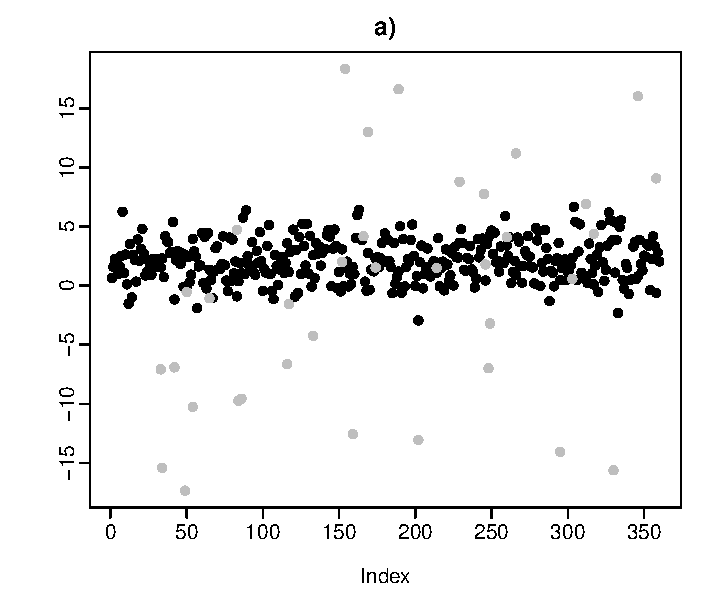
\includegraphics[width=0.32\textwidth]{robflreg-001}
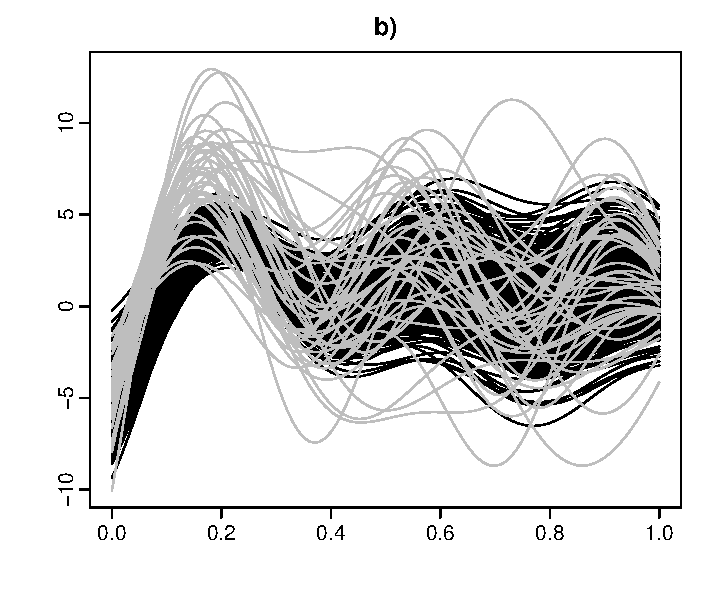
\includegraphics[width=0.32\textwidth]{robflreg-002}
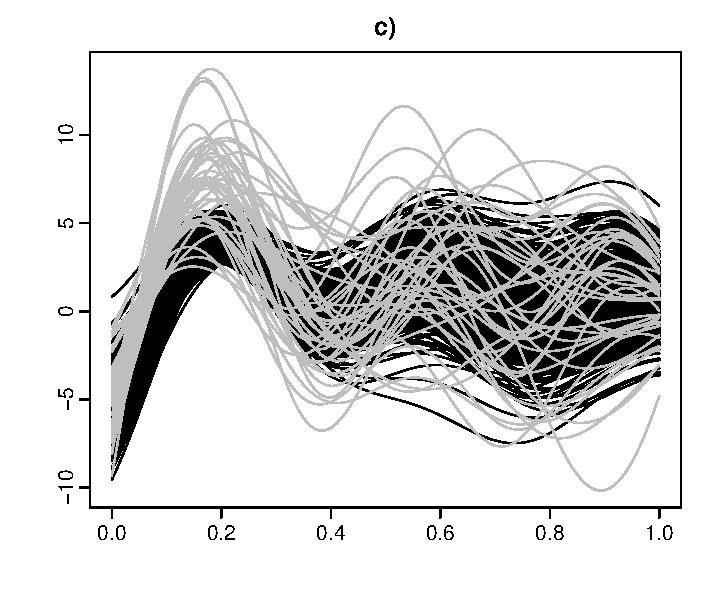
\includegraphics[width=0.32\textwidth]{robflreg-003}\\
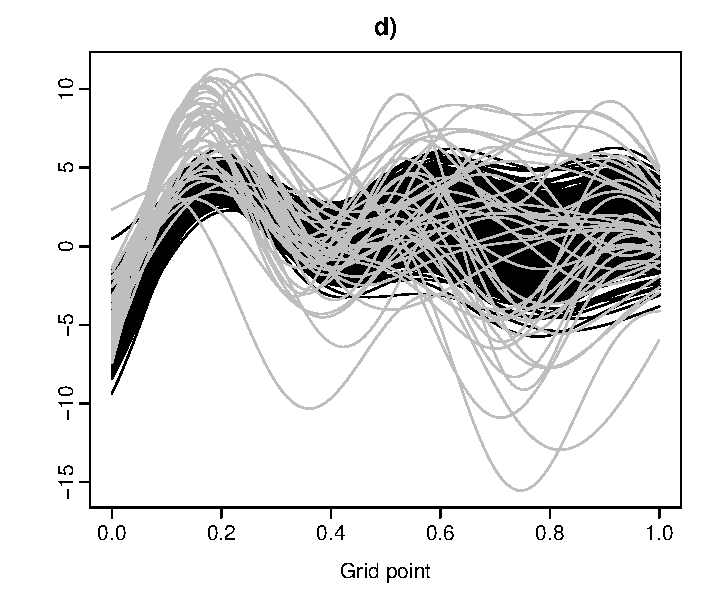
\includegraphics[width=0.32\textwidth]{robflreg-004}
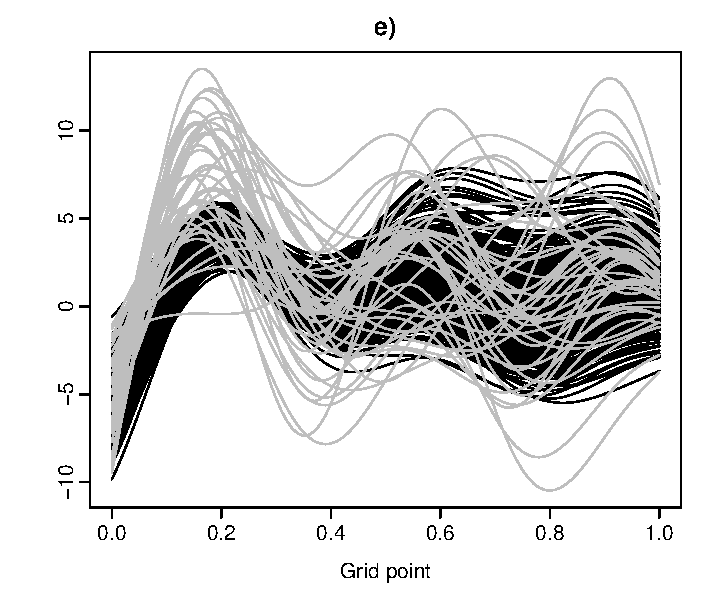
\includegraphics[width=0.32\textwidth]{robflreg-005}
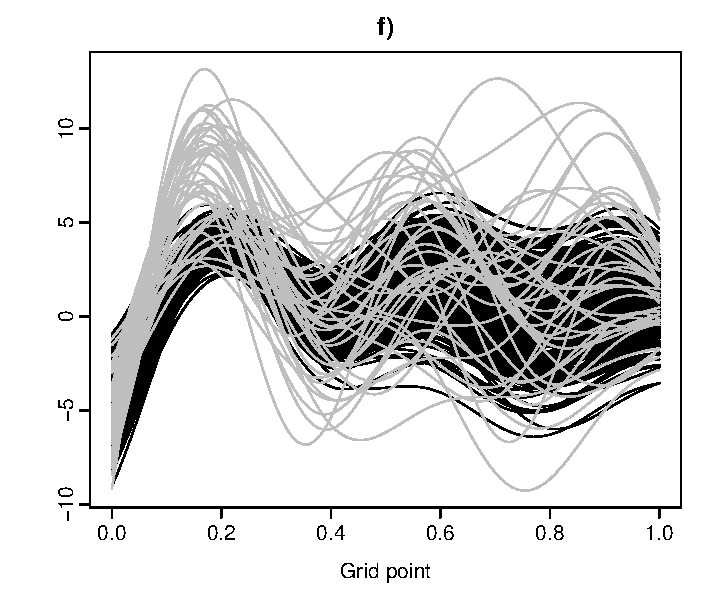
\includegraphics[width=0.32\textwidth]{robflreg-006}
\end{center}
\caption{Plots of the simulated scalar response and the functional predictor variables. a) Observations generated under the main data generating process (black) and outlier points (grey). b-f) Curves of the functional predictors generated under the main data generating process (black) and outlier curves (grey).}\label{fig:1}
\end{figure}

Figure~\ref{fig:1} can be produced by the following code (refer to the supplement code file for all the reproducible code):
\begin{smallexample}
\begin{smallverbatim}
library(robflreg)
library(fda.usc)
set.seed(202)

# Generate a dataset with five functional predictors and 400
# observations at 101 equally spaced point in the interval [0, 1]
# for each variable for the scalar-on-function regression model
sim.data <- generate.sf.data(n = 400, n.pred = 5, n.gp = 101, out.p = 0.1)

# Response variable
Y <- sim.data$Y
# Predictors
X <- sim.data$X
# Regression coefficient functions
coeffs <- sim.data$f.coef
# Plot the scalar response
out.indx <- sim.data$out.indx
plot(Y[-out.indx,], type = "p", pch = 16, xlab = "Index", ylab = "",
main = "Response", ylim = range(Y))
points(out.indx, Y[out.indx,], type = "p", pch = 16, col = "blue")
# Plot the first functional predictor
fX1 <- fdata(X[[1]], argvals = seq(0, 1, length.out = 101))
plot(fX1[-out.indx,], lty = 1, ylab = "", xlab = "", col = "black",
     main = expression(X[1](s)), mgp = c(2, 0.5, 0), ylim = range(fX1))
lines(fX1[out.indx,], lty = 1, col = "grey")
\end{smallverbatim}
\end{smallexample}

\subsection*{The FFLRM}

Let us consider a random sample $\lbrace \mathcal{Y}_i(t), \bm{\mathcal{X}}_i(s)$: $i = 1, 2, \ldots n \rbrace$ from the pair $(\mathcal{Y}, \bm{\mathcal{X}})$, where $\mathcal{Y} \in \mathcal{L}_2 [0,1]$ is the functional response and $\bm{\mathcal{X}} = [\mathcal{X}_1(s), \ldots, \mathcal{X}_P(s)]^\top$ with $\mathcal{X}_p(s) \in \mathcal{L}_2[0,1]$, $\forall~p = 1, \ldots, P$ is the vector of $P$ set of functional predictors. We assume that the functional response and functional predictors have finite second-order moments, i.e., $\text{E}[\Vert \mathcal{Y}(t) \Vert] = \text{E}[\Vert \mathcal{X}_p(s) \Vert] < \infty$, for $p = 1, \ldots, P$. Without loss of generality, we also assume that both $\mathcal{Y}(t)$ and $\mathcal{X}_p(s)$, for $p = 1, \ldots, P$, are mean-zero processes, so that $\text{E}[Y(t)] = \text{E}[\mathcal{X}_p(s)] = 0$. Then, the FFRM is defined as follows:
\begin{equation}\label{eq:fof}
Y_i(t) = \int_0^1 \bm{\mathcal{X}}_i^\top(s) \bm{\beta}(s,t) ds dt + \epsilon_i(t),
\end{equation}
where $\beta_p(s,t) \in \mathcal{L}_2[0,1]$ is the bivariate regression coefficient function linking $\mathcal{Y}(t)$ with $\mathcal{X}_p(s)$, and $\bm{\beta}(s,t) = [ \beta_1(s,t), \ldots, \beta_P(s,t) ]^\top \in \mathcal{L}_2^P[0,1]$, and $\epsilon_i(t) \in \mathcal{L}_2[0,1]$ is the error term which is assumed to be independent of $\mathcal{X}_p(s)$, for $p = 1, \ldots, P$ and $\text{E}[\epsilon_i(t)] = 0$.

\subsubsection*{Simulation of a dataset for the FFLRM}

The function \texttt{generate.ff.data()} allows for the simulation of a dataset for the FFLRM as follows:
\begin{smallexample}
\begin{smallverbatim}
generate.ff.data(n.pred, n.curve, n.gp, out.p = 0)
\end{smallverbatim}
\end{smallexample}
Similar to the \texttt{generate.sf.data()}, \texttt{n.pred} denotes the number of functional predictors to be generated, \texttt{n.curve} denotes the number of observations for each functional variable to be generated, \texttt{n.gp} denotes the number of grid points, and \texttt{out.p} is an integer between 0 and 1, denoting the outlier percentage in the generated data. When generating a dataset, first, the function \texttt{generate.ff.data()} first simulates the functional predictors via the following process:
\begin{equation*}
\mathcal{X}(s) = \sum_{j=1}^5 \kappa_j \nu_j(s),
\end{equation*}
where $\kappa_j$ is a vector generated from a Normal distribution with mean one and variance $\sqrt{a}j^{-1/2}$, where $a$ is is a uniformly generated random number between 1 and 4, and
\begin{equation*}
\nu_j(s) = \sin (j \pi s) - \cos (j \pi s).
\end{equation*}
The bivariate regression coefficient functions are generated from a coefficient space that includes ten different functions such as $b \sin(2 \pi s) \sin(\pi t)$ and $b e^{-3(s-0.5)^2} e^{-4(t-1)^2}$, where $b$ is generated from a uniform distribution between 1 and 3. The error process $\epsilon(t)$, on the other hand, is generated from the Ornstein-Uhlenbeck process:
\begin{equation*}
\epsilon(t) = l + [\epsilon_0(t) - l] e^{-\theta t} \sigma \int_0^t e^{-\theta (t-u)} d W_u,
\end{equation*}
where $l, \theta > 0, \sigma > 0$ are real constants, $\epsilon_0(t)$ is the initial value of $\epsilon(t)$ taken from $W_u$, and $W_u$ is the Wiener process. If outliers are allowed in the generated data, i.e., $out.p > 0$, then, the randomly selected $ n \times out.p$ cases are generated differently from the process mentioned above. In more detail, if $out.p > 0$, the regression coefficient functions (possibly different from the previously generated coefficient functions) generated from the coefficient space with $b^*$ (instead of $b$), where $b^*$ is generated from a uniform distribution between 1 and 2, are used to generate the outlying observations. In addition, in this case, the following process is used to generate functional predictors:
\begin{equation*}
\mathcal{X}^*(s) = \sum_{j=1}^5 \kappa_j^* \nu_j^*(s),
\end{equation*}
where $\kappa_j^*$ is a vector generated from a Normal distribution with mean one and variance $\sqrt{a}j^{-3/2}$ and
\begin{equation*}
\nu_j^*(s) = 2 \sin (j \pi s) - \cos (j \pi s).
\end{equation*}
A graphical display of the generated dataset with five functional predictors and \texttt{n = 200} observations at 101 equally spaced points in the interval $[0, 1]$ obtained by \texttt{generate.ff.data()} is presented in Figure~\ref{fig:2}. 
\begin{figure}[!htb]
  \begin{center}
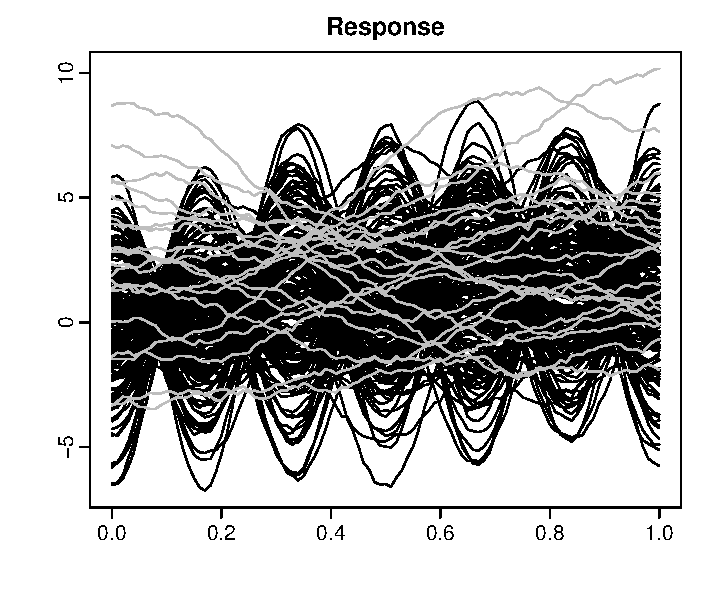
\includegraphics[width=0.32\textwidth]{robflreg-007}
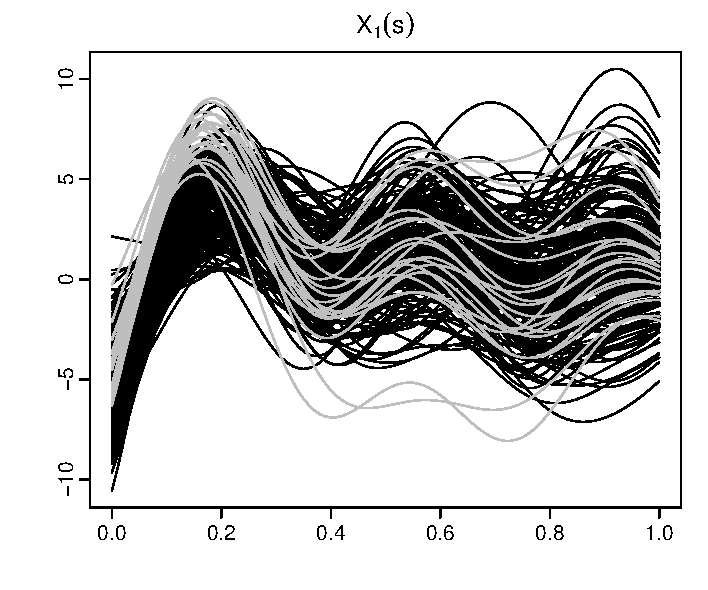
\includegraphics[width=0.32\textwidth]{robflreg-008}
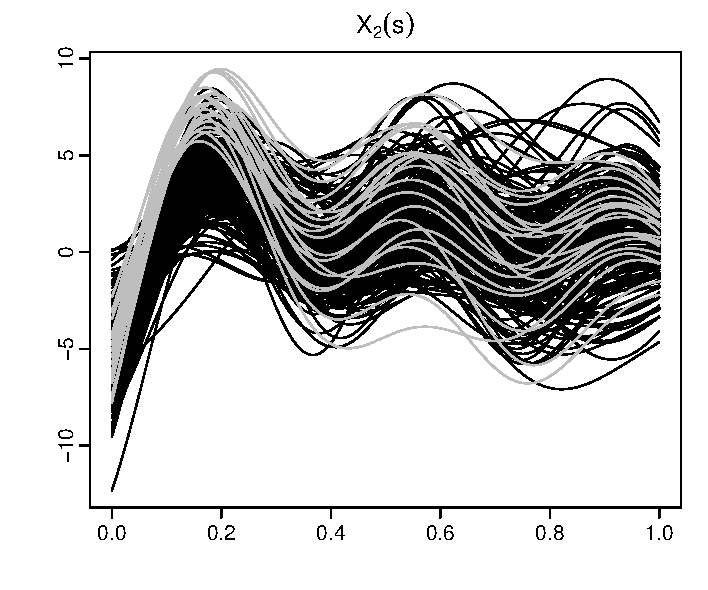
\includegraphics[width=0.32\textwidth]{robflreg-009}\\
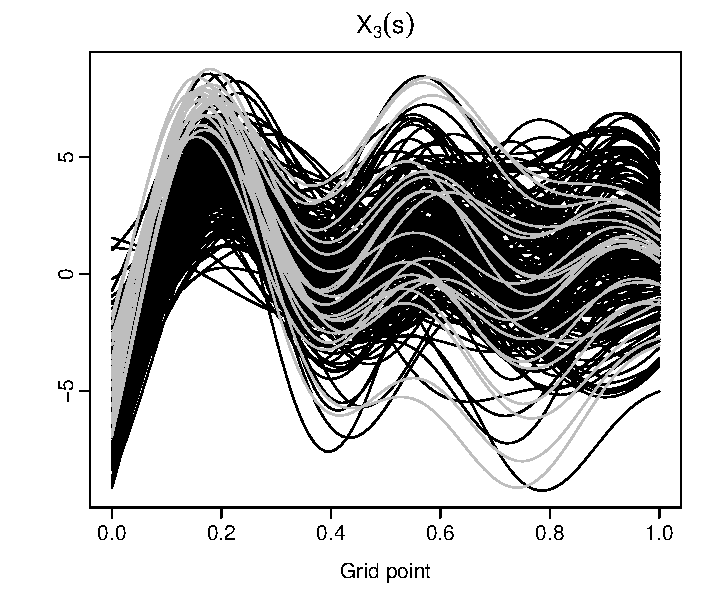
\includegraphics[width=0.32\textwidth]{robflreg-010}
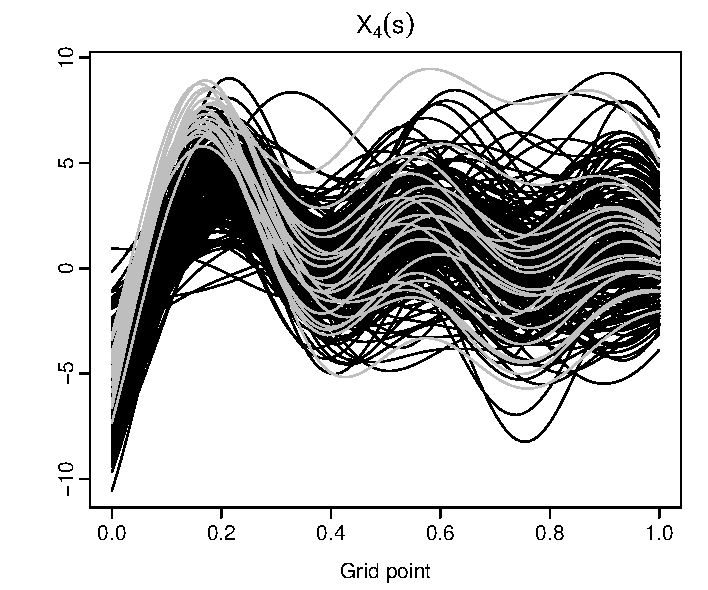
\includegraphics[width=0.32\textwidth]{robflreg-011}
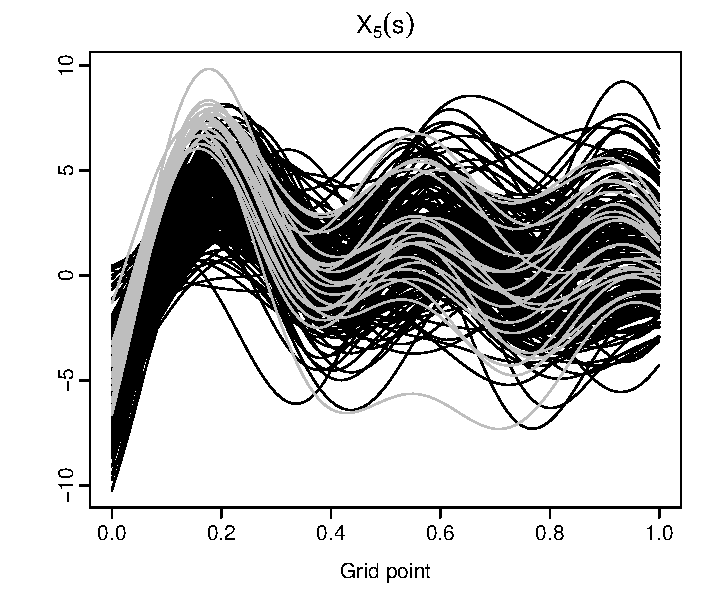
\includegraphics[width=0.32\textwidth]{robflreg-012}
\end{center}
\caption{Plots of the simulated functional response and functional predictor variables: In the plots, the black curves denote the observations of the response and functional predictors generated under the smooth data generation process. The grey curves denote the outlying observations in the functional variables.}\label{fig:2}
\end{figure}

Figure~\ref{fig:2} can be produced by the following code (refer to the supplement code file for all the reproducible code):
\begin{smallexample}
\begin{smallverbatim}
library(robflreg)
library(fda.usc)
set.seed(202)

# Generate a dataset with five functional predictors and 200
# observations at 101 equally spaced point in the interval [0, 1]
# for each variable for the function-on-function regression model
sim.data <- generate.ff.data(n.pred = 5, n.curve = 200, n.gp = 101, out.p = 0.1)

# Response variable
Y <- sim.data$Y
# Predictors
X <- sim.data$X
# Regression coefficient functions
coeffs <- sim.data$f.coef
# Plot the scalar response
out.indx <- sim.data$out.indx
fY <- fdata(Y, argvals = seq(0, 1, length.out = 101))
plot(fY[-out.indx,], lty = 1, ylab = "", xlab = "",
main = "Response", mgp = c(2, 0.5, 0), ylim = range(fY))
lines(fY[out.indx,], lty = 1, col = "grey")
# Plot the first functional predictor
fX1 <- fdata(X[[1]], argvals = seq(0, 1, length.out = 101))
plot(fX1[-out.indx,], lty = 1, ylab = "", xlab = "", col = "black",
main = expression(X[1](s)), mgp = c(2, 0.5, 0), ylim = range(fX1))
lines(fX1[out.indx,], lty = 1, col = "grey")
\end{smallverbatim}
\end{smallexample}

\section{Estimation}

We first review the classical and robust FPCA methods. Then, we will focus on the robust estimation of the SFLRM and FFLRM by the functional principal component regression.

\subsection*{Functional principal component analysis (FPCA)}

For a functional random variable $\mathcal{X}(s)$, let us denote its covariance function by $\mathcal{C}(s_1, s_2) = \text{Cov}[\mathcal{X}(s_1),~\mathcal{X}(s_2)]$ satisfying $\int_0^1 \int_0^1 \mathcal{C}(s_1, s_2) ds_1 ds_2 < \infty$. Then, by Mercer's Theorem, the following representation holds:
\begin{equation*}
\mathcal{C} = \sum_{k=1}^{\infty} \kappa_k \psi_k(s_1) \psi_k(s_2), \quad \forall s_1, s_2 \in [0,1],
\end{equation*}
where $\left \lbrace \psi_k(s): k = 1, 2, \ldots \right \rbrace$ are orthonormal bases of eigenfunctions in $\mathcal{L}_2[0,1]$ corresponding to the non-negative eigenvalues $\left \lbrace \kappa_k: k = 1, 2, \ldots \right \rbrace$ with $\kappa_k \geq \kappa_{k+1}$. In practice, most of the variability in functional variables can be captured via a finite number of the first $K$ eigenfunctions. Thus, the covariance function of a functional variable is estimated using a pre-determined truncation constant $K$. In addition, the orthonormal bases of eigenfunctions are unknown in practice. Thus, they are approximated via a suitable basis expansion method such as B-spline, which is used in the \pkg{robflreg} package.

The RFPCA of \cite{Bali2011} follows a similar structure as the classical FPCA, but it uses a robust scale functional instead of variance. Now let $\Vert \alpha \Vert^2 = \langle \alpha, \alpha \rangle$ denote the norm generated by the inner product $\langle \cdot, \cdot \rangle$. Also, let $\mathcal{F}[\alpha]$ denote the distribution of $\langle \alpha, \mathcal{X} \rangle$ where $\mathcal{F}$ is the distribution of $\mathcal{X}$. Then, for a given M-scale functional $\sigma_M(\mathcal{F})$, the orthonormal bases of eigenfunctions defined by \cite{Bali2011} are as follows:
\[ \begin{cases}
\psi_k(\mathcal{F}) = \underset{\begin{subarray}{c}
      \Vert \alpha \Vert^2 = 1
\end{subarray}}{\arg \max}~ \sigma_M(\mathcal{F}[\alpha]), & k = 1, \\
\psi_k(\mathcal{F}) = \underset{\begin{subarray}{c}
      \Vert \alpha \Vert^2 = 1, \alpha \in \mathcal{B}_k
\end{subarray}}{\arg \max}~ \sigma_M(\mathcal{F}[\alpha]), & k \geq 2,
   \end{cases}
\]
where $\mathcal{B}_k = \left\lbrace \alpha \in \mathcal{L}_2[0,1]: \langle \alpha, \psi_k ( \mathcal{F} ) \rangle = 0, ~ 1 \leq k \leq \ K - 1 \right\rbrace$. The $k$-th largest eigenvalue is given by:
\begin{equation*}
\kappa_k(\mathcal{F}) = \sigma_M^2(\mathcal{F}[\psi_k]) = \underset{\begin{subarray}{c}
      \Vert \alpha \Vert^2 = 1, \alpha \in \mathcal{B}_k
\end{subarray}}{\max} \sigma_M^2(\mathcal{F}[\alpha]).
\end{equation*}

Denote by $\sigma_M(\mathcal{F}_n[\alpha])$ the functional for $\sigma_M$. Let $s^2_n: \mathcal{L}_2[0,1] \rightarrow \mathbb{R}$ denote the function of empirical M-scale functional such that $s^2(\alpha) = \sigma_M^2(\mathcal{F}[\alpha])$. Then, the RFPCA estimates of the orthonormal bases of eigenfunctions for $\mathcal{X}(s)$ are given by
\[ \begin{cases}
\widehat{\psi}_k(s) = \underset{\begin{subarray}{c}
      \Vert \alpha \Vert^2 = 1
\end{subarray}}{\arg \max}~ s_n(\alpha), & k = 1, \\
\widehat{\psi}_k(s) = \underset{\begin{subarray}{c}
      \alpha \in \widehat{\mathcal{B}}_k
\end{subarray}}{\arg \max}~ s_n(\alpha), & k \geq 2,
   \end{cases}
\]
where $\widehat{\mathcal{B}}_k = \left\lbrace \alpha \in \mathcal{L}_2 [0,1]: \Vert \alpha \Vert = 1, \langle \alpha, \widehat{\psi}_k \rangle = 0, ~ \forall~ 1 \leq k \leq \ K - 1 \right\rbrace$. The corresponding eigenvalues, on the other hand, are given by
\begin{equation*}
\widehat{\kappa}_k = s^2_n (\widehat{\psi}_k), \quad k \geq 1.
\end{equation*}

\subsubsection*{Main RFPCA function and its arguments}

The main function to obtain the robust estimates of functional principal components and the corresponding principal component scores is called \texttt{getPCA()}:
\begin{smallexample}
\begin{smallverbatim}
getPCA(data, nbasis, ncomp, gp, emodel = c("classical", "robust"))
\end{smallverbatim}
\end{smallexample}
In the \texttt{getPCA()} function, the data set is provided in the \texttt{data} argument as a matrix. The grid points of the functional predictors are provided in the \texttt{gp} argument as a vector. \texttt{nbasis} denotes the number of B-spline basis expansion functions used to approximate the robust functional principal components. \texttt{ncomp} specifies the number of functional principal components to be computed. The argument \texttt{emodel} denotes the method used for functional principal component decomposition. If \texttt{emodel = "classical"}, then the classical functional principal component decomposition is performed. On the other hand, if \texttt{emodel = "robust"}, then the RFPCA method of \cite{Bali2011} is used to obtain the functional principal components and the corresponding principal component scores. Figure~\ref{fig:3} presents the plot of five functional principal components computed from simulated functional data using RFPCA and \texttt{nbasis = 20} B-spline basis expansion functions. 
\begin{figure}[!htb]
  \begin{center}
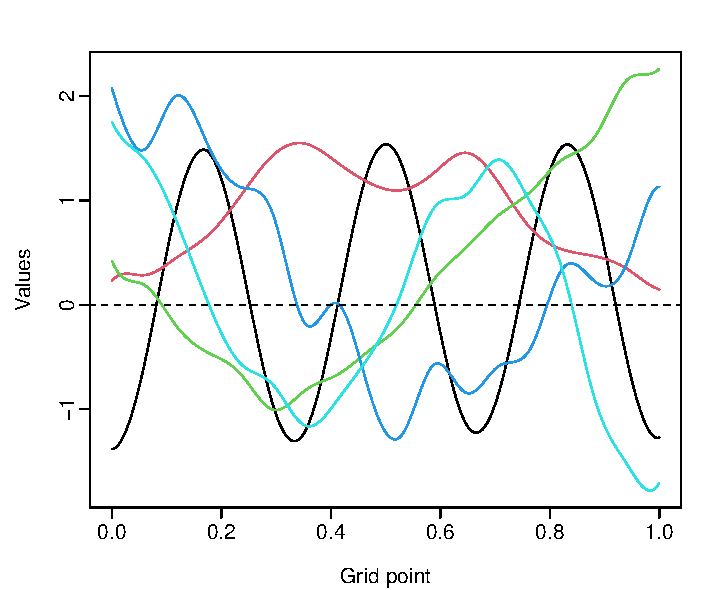
\includegraphics[width=0.6\textwidth]{robflreg-013}
\end{center}
\caption{Plot of the first five functional principal components of the simulated functional data. The principal components were obtained using the RFPCA and different colors correspond to different principal components.}\label{fig:3}
\end{figure}

Figure~\ref{fig:3} can be produced by the following code:
\begin{smallexample}
\begin{smallverbatim}
library(robflreg)
# Generate a dataset with five functional predictors and 200
# observations at 101 equally spaced point in the interval [0, 1]
# for each variable for the function-on-function regression model
set.seed(202)
sim.data <- generate.ff.data(n.pred = 5, n.curve = 200, n.gp = 101)
# Response variable
Y <- sim.data$Y
gpY <- seq(0, 1, length.out = 101) # grid points

# Perform robust functional principal component analysis on the response variable Y
rob.fpca <- getPCA(data = Y, nbasis = 20, ncomp = 5, gp = gpY, emodel = "robust")

# Principal components
PCs <- rob.fpca$PCAcoef

plot(PCs, xlab = "Grid point", ylab = "Values", lty = 1)
\end{smallverbatim}
\end{smallexample}


\subsection*{Robust estimation of the SFLRM}

In the robust estimation of the SFRM, we first consider the principal component decomposition of the functional predictors as follows:
\begin{equation*}
\mathcal{X}_p(s) = \sum_{k=1}^{K_p} \xi_{pk} \psi_{pk}(s),
\end{equation*}
where $K_p$ is the truncation constant for the $p$-th functional predictor $\mathcal{X}_p(s)$, $\psi_{pk}(s)$ is the $k$-th eigenfunction obtained by the RFPCA of \cite{Bali2011}, and $\xi_{pk}$ is the corresponding principal component score, given by:
\begin{equation*}
\xi_{pk} = \int_0^1 \mathcal{X}_p(s) \psi_{pk}(s) ds.
\end{equation*}

In practice, the eigenfunctions are approximated via a basis expansion function such as B-spline. Let $\varphi_p(s)$ denote the B-spline basis expansion function, and $A_p = (a_{pl})$ be an $n \times L$-dimensional matrix of basis expansion coefficients for the $p$-th functional predictor variable. In addition, let $\bm{\varphi} = \int_0^1 \varphi_p(s) \varphi_p^\top (s) ds$ and $\bm{\varphi}^{1/2}$ denote the $L \times L$ dimensional matrix of inner products between the basis expansion functions and its square root, respectively. Then, the infinite-dimensional RFPCA of $\mathcal{X}_p(s)$ is equivalent to the multivariate principal component analysis of $A_p \bm{\varphi}^{1/2}$ and the $k$-th eigenfunction is given by $\psi_{pk}(s) = \bm{\varphi}^{-1/2} v_{pk}$, where $v_{pk}$ denotes the $p$-th eigenvector of the sample covariance matrix of $A_p \bm{\varphi}^{1/2}$ \citep[see, e.g.,][for more information]{Ocana2007}.

If we assume that the $p$-th regression coefficient function $\beta_p(s)$ admits the similar functional principal decomposition as the functional predictors as follows:
\begin{equation*}
\beta_p(s) = \sum_{k=1}^{K_p} b_{pk} \psi_{pk}(s),
\end{equation*}
where $b_{pk} = \int_0^1 \beta_p(s) \psi_{pk}(s) ds$. Then, the infinite-dimensional SFRM in~\eqref{eq:sof} is approximated by the finite-dimensional regression model of scalar response on all the functional principal component scores as follows:
\begin{equation*}
Y = \sum_{p=1}^P \sum_{k=1}^{K_p} b_{pk} \xi_{pk}.
\end{equation*}

\subsubsection*{Main functions for the robust estimation of a SFRM and their arguments}

The main function for robust estimation of SFRMs is called \texttt{rob.sf.reg()}:
\begin{smallexample}
\begin{smallverbatim}
rob.sf.reg(Y, X, X.scl = NULL, emodel = c("classical", "robust"),
fmodel = c("LTS", "MM", "S", "tau"), nbasis = NULL, gp = NULL, ncomp = NULL)
\end{smallverbatim}
\end{smallexample}

In the \texttt{rob.sf.reg()} function, the scalar response is provided in the \texttt{Y} argument as an $n \times 1$-dimensional column vector, where $n$ is the sample size. The functional predictors, on the other hand, are provided as a list object in the \texttt{X} argument. Each element of \texttt{X} is an $n \times L_p$-dimensional matrix containing the observations of $p$-th functional predictor $\mathcal{X}_p(s)$, where $L_p$ is the number of grid points for $\mathcal{X}_p(s)$. The \texttt{rob.sf.reg()} function also allows for scalar predictors, which can be provided in the \texttt{X.scl} as an $n \times R$-dimensional matrix, where $R$ denotes the number of scalar predictors. In this case, the following SFRM is considered:
\begin{equation*}
Y_i = \int_0^1 \bm{\mathcal{X}}_i^\top(s) \bm{\beta}(s) ds + \text{X.scl}_i \bm{\gamma} + \epsilon_i,
\end{equation*}
where $\bm{\gamma}$ denotes the vector of coefficients for the scalar predictors' matrix. The functional principal component decomposition method is provided in the \texttt{emodel} argument. If \texttt{emodel = "classical"}, then the classical functional principal component decomposition is performed to obtain principal components and the corresponding principal component scores. The coefficient vector of the regression problem of scalar response on the principal component scores is estimated via the least-squares method. If \texttt{emodel = "robust"}, then the RFPCA of \cite{Bali2011} is performed to obtain the principal components and the corresponding principal component scores. In this case, the method used to estimate the coefficient vector of the regression problem constructed by the scalar response and principal component scores is provided in the \texttt{fmodel} argument. One of the methods among LTS, MM, S, and tau can be chosen to estimate the parameter vector (by specifying, for example, fmodel = tau"). The number of B-spline basis expansion functions used to approximate the functional principal components are provided in the \texttt{nbasis} argument as a vector with length $p$. Suppose \texttt{nbasis = NULL}, then $\min(20, L_p / 4)$ number of B-spline basis expansion functions are used for each functional predictor. The grid points for the functional predictors are provided in the \texttt{gp} argument as a list object. The $p$-th element of \texttt{gp} is a vector containing the grid points of the $p$-th functional predictor $\mathcal{X}_p(s)$. If \texttt{gp = NULL}, then $L_p$ equally spaced time points in the interval $[0,1]$ are used for the $p$-th functional predictor. The number of principal components to be computed for the functional predictors are provided in the \texttt{ncomp} argument as a vector with length $P$. If \texttt{ncomp = NULL}, then, for each functional predictor, the number whose usage results in at least 95\% explained variation is used as the number of principal components.

The function \texttt{get.sf.coeffs()} can be used to obtain the estimated regression coefficient functions from a fitted functional principal component regression:
\begin{smallexample}
\begin{smallverbatim}
get.sf.coeffs(object)
\end{smallverbatim}
\end{smallexample}
In this function, the argument \texttt{object} is the output object obtained using the function \texttt{rob.sf.reg()}. The function \texttt{get.sf.coeffs()} produces a list object whose $p$-th element is a vector with length $L_p$ containing the $p$-th regression coefficient function $\beta_p(s)$.

The plots of the estimated regression coefficient functions can be obtained using the function \texttt{plot\_sf\_coeffs()}:
\begin{smallexample}
\begin{smallverbatim}
plot_sf_coeffs(object, b)
\end{smallverbatim}
\end{smallexample}
In Figure~\ref{fig:4}, the plots of the regression coefficient functions obtained from simulated data (outlier-contaminated) using \texttt{RFPCA} and MM estimator, as well as the classical functional principal component regression, are presented. In this function, the argument \texttt{object} is the output object obtained by the function \texttt{get.sf.coeffs()}. On the other hand, the argument \texttt{b} is an integer value indicating which regression parameter function to plot. It is clear from this figure that, compared with the classical functional principal component regression, the robust approach produces estimated parameter functions which are more similar to the true  parameter functions.
\begin{figure}[!htb]
  \begin{center}
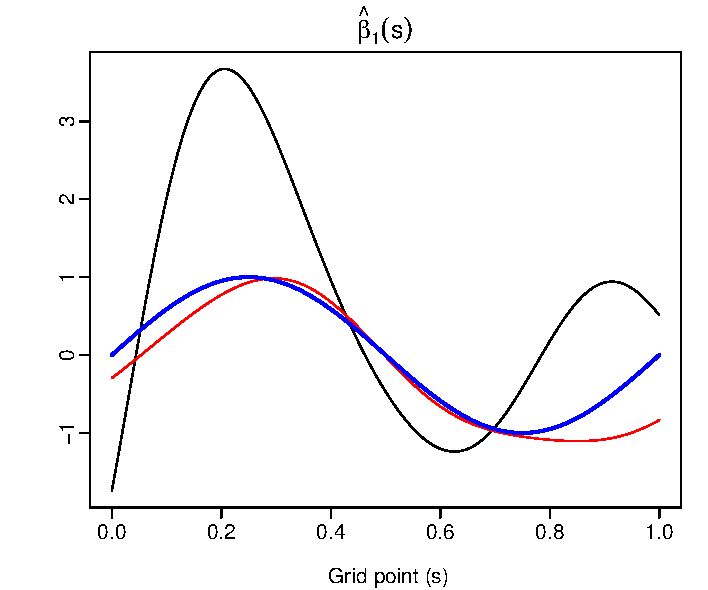
\includegraphics[width=0.32\textwidth]{robflreg-014}
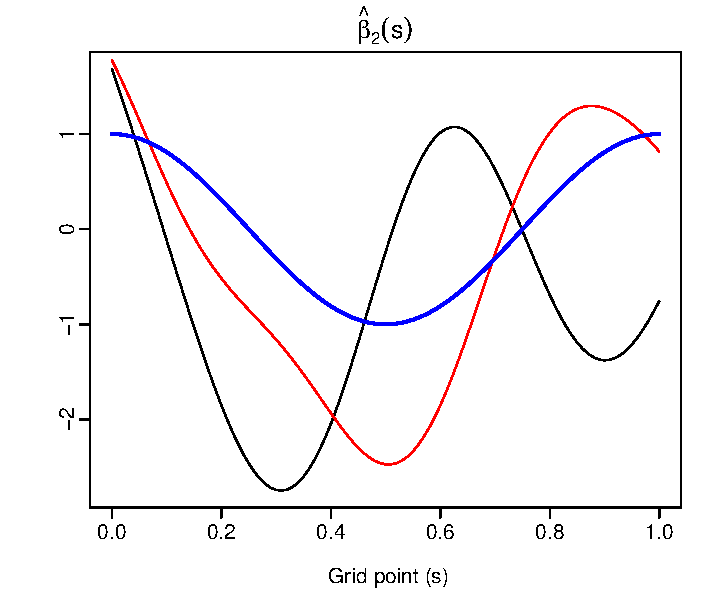
\includegraphics[width=0.32\textwidth]{robflreg-015}
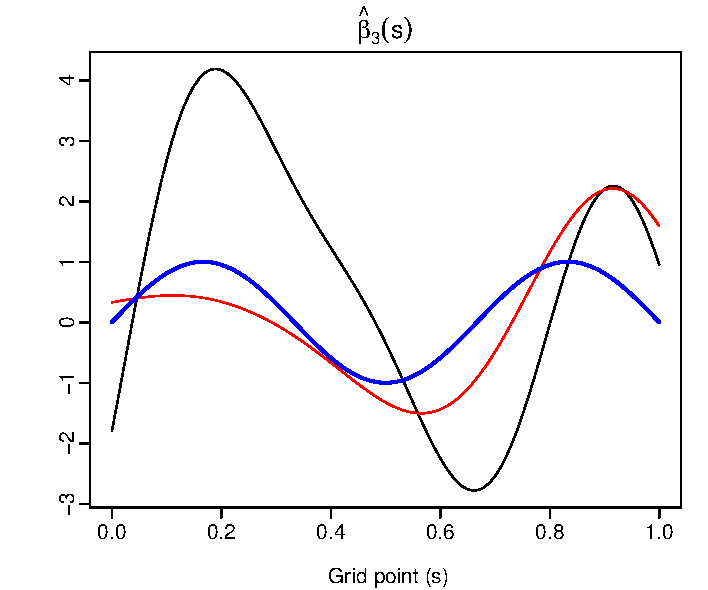
\includegraphics[width=0.32\textwidth]{robflreg-016}
\end{center}
\caption{A plot of the estimated regression coefficient functions obtained from simulated data (outlier-contaminated) using RFPCA and MM estimator and the classical functional principal component regression. Blue lines denote the true parameter functions. On the other hand, black and red lines denote the estimated parameter functions by the classical functional principal component regression and robust MM-based functional principal component regression, respectively.}\label{fig:4}
\end{figure}

The following code can be used to produce this figure and the results (refer to the supplement code file for all of the reproducible code):
\begin{smallexample}
\begin{smallverbatim}
library(robflreg)
# Generate a dataset with three functional predictors and 400
# observations at 101 equally spaced point in the interval [0, 1]
# for each variable for the scalar-on-function regression model
set.seed(202)
sim.data <- generate.sf.data(n = 400, n.pred = 3, n.gp = 101, out.p = 0.1)

# True parameter functions
true.b1 <- sim.data\$f.coef[[1]]
true.b2 <- sim.data\$f.coef[[2]]
true.b3 <- sim.data\$f.coef[[3]]

# Response variable
Y <- sim.data\$Y
# Predictors
X <- sim.data\$X

gp <- rep(list(seq(0, 1, length.out = 101)), 3) # grid points of Xs

# Fit a functional principal component regression model for the generated data
# using the classical functional principal component analysis method:
classical.fit <- rob.sf.reg(Y, X, emodel = "classical", gp = gp)

# Fit a functional principal component regression model for the generated data
# using the robust functional principal component analysis method and tau estimator:
robust.fit <- rob.sf.reg(Y, X, emodel = "robust", fmodel = "MM", gp = gp)

# Estimated regression coefficient functions
classical.coefs <- get.sf.coeffs(classical.fit)
robust.coefs <- get.sf.coeffs(robust.fit)

# The first estimated regression coefficient function
plot_sf_coeffs(object = classical.coefs, b = 1)
lines(gp[[1]], robust.coefs\$coefficients[[1]], col = "red")
lines(gp[[1]], true.b1, col = "blue", lwd = 2)
\end{smallverbatim}
\end{smallexample}

\subsection*{Robust estimation of the FFLRM}

Let us consider the functional principal decompositions of both the functional response and functional predictor variables as follows:
\begin{equation*}
\mathcal{Y}(t) = \sum_{k=1}^K \zeta_k \phi_k(t), \quad \mathcal{X}_p(s) = \sum_{j=1}^{K_p} \xi_{pj} \psi_{pj}(s),
\end{equation*}
where $\phi_k(t)$ and $\psi_{pj}(s)$ respectively are the $k$-th and $j$-th eigenfunctions of $\mathcal{Y}(t)$ and $\mathcal{X}_p(s)$ obtained by the RFPCA and $\zeta_k$ and $\xi_{pj}$ are the corresponding principal component scores given by
\begin{equation*}
\zeta_k = \int_0^1 \mathcal{Y}(t) \phi_k(t) dt, \quad \xi_{pj} = \int_0^1 \mathcal{X}_p(s) \psi_{pj}(s) ds.
\end{equation*}
If we assume that the $p$-th bivariate regression coefficient function $\beta_p(s,t)$ admits the principal component decomposition with the eigenfunctions $\phi_k(t)$ and $\psi_{pj}(s)$ as follows:
\begin{equation*}
\beta_p(s,t) = \sum_{k=1}^K \sum_{j=1}^{K_p} b_{pkj} \phi_k(t) \psi_{pj}(s),
\end{equation*}
where $b_{pkj} = \int_0^1 \int_0^1 \beta_p(s,t) \phi_k(t) \psi_{pj}(s) dt ds$. Then, the infinite-dimensional FFRM in~\eqref{eq:fof} is approximated by the finite-dimensional regression model of principal component scores of the functional response on all the functional principal component scores as follows:
\begin{equation*}
\zeta_k = \sum_{p=1}^P \sum_{j=1}^{K_p} b_{pkj} \xi_{pj}.
\end{equation*}
Finally, the following regression model is obtained for the functional response
\begin{equation*}
\mathcal{Y}(t) = \sum_{k=1}^K \left(\sum_{p=1}^P \sum_{j=1}^{K_p} b_{pkj} \xi_{pj} \right) \phi_k(t).
\end{equation*}

\subsubsection*{Main functions for the robust estimation of a FFRM and their arguments}

The main function to estimate the FFRM robustly is called \texttt{rob.ff.reg()}:
\begin{smallexample}
\begin{smallverbatim}
rob.ff.reg(Y, X, model = c("full", "selected"), emodel = c("classical", "robust"),
fmodel = c("MCD", "MLTS", "MM", "S", "tau"), nbasisY = NULL, nbasisX = NULL,
gpY = NULL, gpX = NULL, ncompY = NULL, ncompX = NULL)
\end{smallverbatim}
\end{smallexample}

In the \texttt{rob.ff.reg()} function, the functional response is provided via the \texttt{Y} argument as a matrix. On the other hand, the functional predictors are provided in the argument \texttt{X} as a list object. Each element of \texttt{X} is a matrix containing the observations of $p$-th functional predictor. The model type to be fitted can be chosen with \texttt{model} argument. If \texttt{model = "full"}, then all of the functional predictors are used in the model. On the other hand, if \texttt{model = "selected"}, then only the significant functional predictor variables, determined by the forward variable selection procedure of \cite{BS22}, are used in the model. The functional principal component decomposition method is provided via the \texttt{emodel} argument. If \texttt{emodel = "classical"}, then the classical functional principal component decomposition is performed to obtain principal components and the corresponding principal component scores and the coefficient vector of the regression problem of principal component scores of the functional response on the principal component scores are estimated via the least-squares method. If \texttt{emodel = "robust"}, then the RFPCA of \cite{Bali2011} is performed to obtain the principal components and the corresponding principal component scores. In this case, the method used to estimate the coefficient matrix of the regression problem constructed by the principal component scores is provided in the \texttt{fmodel} argument. Here, one of the methods, among MCD, MLTS, MM, S, and tau estimators, can be chosen to estimate the parameter matrix. The number of B-spline basis expansion functions used to approximate the functional principal components of response and predictor variables are provided in the \texttt{nbasisY} and \texttt{nbasisX} arguments, respectively. The argument \texttt{nbasisY} is a numeric value while the argument \texttt{nbasisX} is a vector with length $P$. Suppose \texttt{nbasisY = NULL} and \texttt{nbasisX = NULL}, then $\min(20, L_y)$ and $\min(20, L_p)$ B-spline basis expansion functions are used to approximate the functional principal components of functional response and $p$-th the functional predictor, where $L_y$ and $L_p$ respectively denote the number of grid points for $\mathcal{Y}(t)$ and $\mathcal{X}_p(s)$. The grid points for the functional response and functional predictors are provided in the \texttt{gpY} and \texttt{gpX} arguments, respectively. The argument \texttt{gpY} is a vector consisting of the grid points of the functional response $\mathcal{Y}(t)$. On the other hand, the argument \texttt{gpX} is a list object, and its $p$-th element is a vector containing the grid points of the $p$-th functional predictor $\mathcal{X}_p(s)$. If \texttt{gpY = NULL} and If \texttt{gpX = NULL}, then equally spaced time points in the interval $[0,1]$ are used for all the functional variables. The number of functional predictors to be computed for the functional response and functional predictors are provided in the arguments \texttt{ncompY} and \texttt{ncompX}, respectively. The argument \texttt{ncompY} is a numeric value while the argument \texttt{ncompX} is a vector with length $P$. If \texttt{ncompY = NULL} and \texttt{ncompX = NULL}, then the number whose usage results in at least 95\% explained variation is used as the number of principal components for each functional variable.

The estimated bivariate regression coefficient functions from a fitted functional principal component regression model are obtained by the \texttt{get.ff.coeffs()} function:
\begin{smallexample}
\begin{smallverbatim}
get.ff.coeffs(object)
\end{smallverbatim}
\end{smallexample}
In this function, the argument \texttt{object} is the output object obtained using the function \texttt{rob.ff.reg()}. The function \texttt{get.ff.coeffs()} produces a list object whose $p$-th element is a matrix containing the $p$-th bivariate regression coefficient function $\beta_p(s,t)$.

The image plots of the estimated bivariate regression coefficient functions can be obtained using the function \texttt{plot\_ff\_coeffs()}:
\begin{smallexample}
\begin{smallverbatim}
plot_ff_coeffs(object, b)
\end{smallverbatim}
\end{smallexample}
In Figure~\ref{fig:5}, the image plots of the regression coefficient functions obtained from simulated data using \texttt{RFPCA} and MM estimator are presented. In this function, the argument \texttt{object} is the output object obtained by the function \texttt{get.ff.coeffs()}. The argument \texttt{b} is an integer value indicating which regression parameter function is to be plotted.
\begin{figure}[!htb]
  \begin{center}
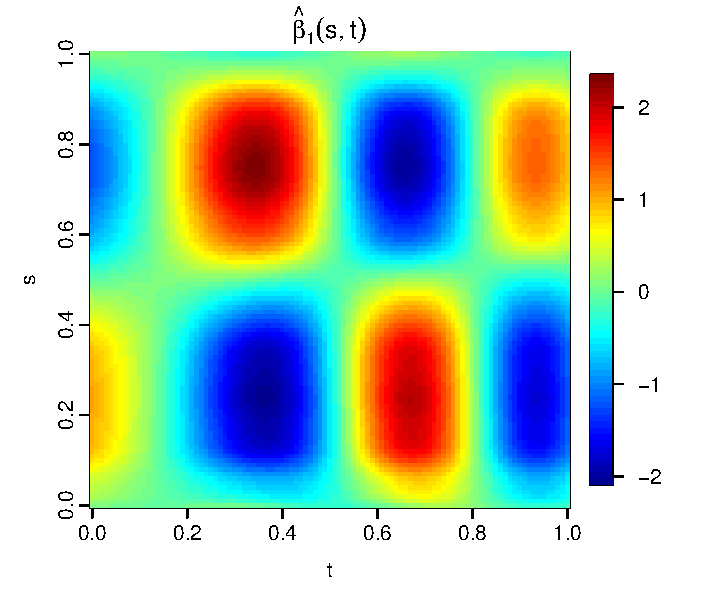
\includegraphics[width=0.32\textwidth]{robflreg-017}
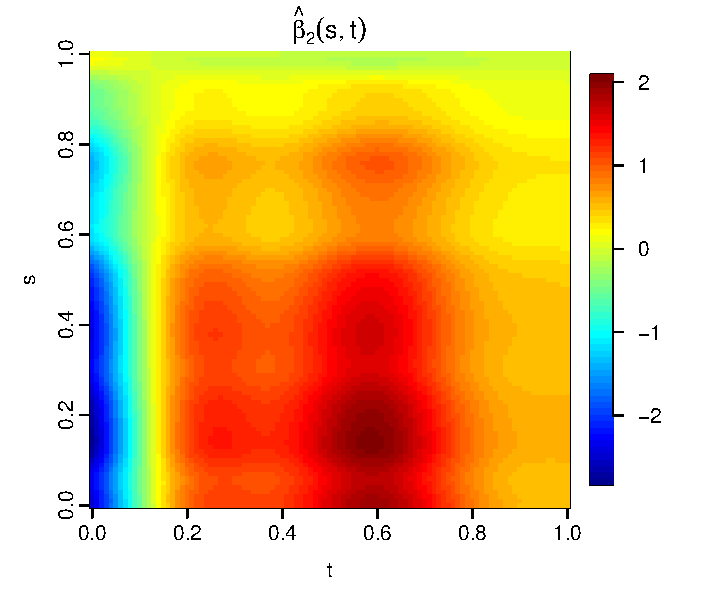
\includegraphics[width=0.32\textwidth]{robflreg-018}
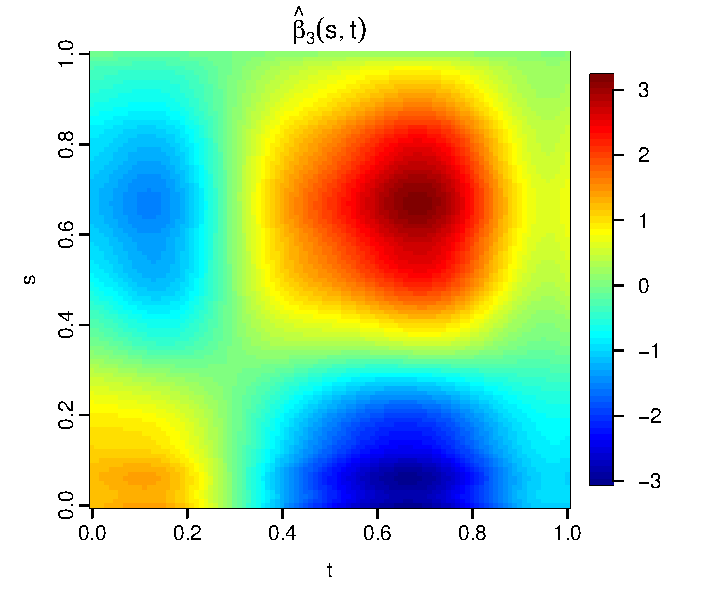
\includegraphics[width=0.32\textwidth]{robflreg-019}
\end{center}
\caption{Image plots of the estimated bivariate regression coefficient functions obtained from simulated data using RFPCA and MM estimator.}\label{fig:5}
\end{figure}

This figure and the results can be produced by the following code (refer to the supplement code file for all the reproducible code):
\begin{smallexample}
\begin{smallverbatim}
library(robflreg)
# Generate a dataset with three functional predictors and 200
# observations at 101 equally spaced point in the interval [0, 1]
# for each variable for the function-on-function regression model
set.seed(202)
sim.data <- generate.ff.data(n.pred = 3, n.curve = 200, n.gp = 101)
# Response variable
Y <- sim.data$Y
# Predictors
X <- sim.data$X

gpY = seq(0, 1, length.out = 101) # grid points of Y
gpX <- rep(list(seq(0, 1, length.out = 101)), 3) # grid points of Xs

# Fit a functional principal component regression model for the generated data
# using the RFPCA and MM estimator:
model.fit <- rob.ff.reg(Y, X, model = "full", emodel = "robust",
fmodel = "MM", gpY = gpY, gpX = gpX)

# Estimated bivariate regression coefficient functions
coefs <- get.ff.coeffs(model.fit)
# Plot the first bivariate regression coefficient function
plot_ff_coeffs(object = coefs, b = 1)
\end{smallverbatim}
\end{smallexample}

\subsubsection*{Outlier detection in the functional response}

Detection of outliers in functional data is an important problem \citep[see, e.g.,][]{Sun2011, Aribas2014, Dai2018}. From a fitted functional principal component regression for scalar response and scalar predictors, the \pkg{robflr} package with the function \texttt{rob.out.detect()} allows to detection of outliers in the functional response. This is achieved by applying the function depth-based outlier detection method of \cite{Febrero08} together with the h-modal depth proposed by \cite{cuevas07} to the estimated residual functions obtained from \texttt{rob.ff.reg()} to determine the outliers in the response variable. In the outlier detection algorithm, the threshold value used to identify outliers is determined by the smoothed bootstrap procedure proposed by \cite{Febrero08}. The \texttt{rob.out.detect()} is as follows:
\begin{smallexample}
\begin{smallverbatim}
rob.out.detect(object, alpha = 0.01, B = 200, fplot = FALSE)
\end{smallverbatim}
\end{smallexample}
Herein, the argument  \texttt{object} is an output object obtained from \texttt{rob.ff.reg()}. \texttt{alpha}, whose default value is 0.01, denotes the percentile of the distribution of the functional depth. \texttt{B} denotes the number of bootstrap samples (the default value is \texttt{B = 200}). \texttt{fplot} is a logical argument, if \texttt{fplot = TRUE}, then the outlying points flagged by the method are plotted along with the values of functional response $\mathcal{Y}(t)$.

To show how the function \texttt{rob.ff.reg()} works, we simulate an outlier-contaminated dataset for the FFRM. Then, we apply the outlier detection algorithm with the classical FPCA - least squares estimator and the RFPCA - MM estimator. The plots of the functional response and detected outlying observations are presented in Figure~\ref{fig:6}. The results show that the classical method fails to flag 13 outlying curves, while the robust procedure fails to flag only two outlying curves. 
\begin{figure}[!htb]
  \begin{center}
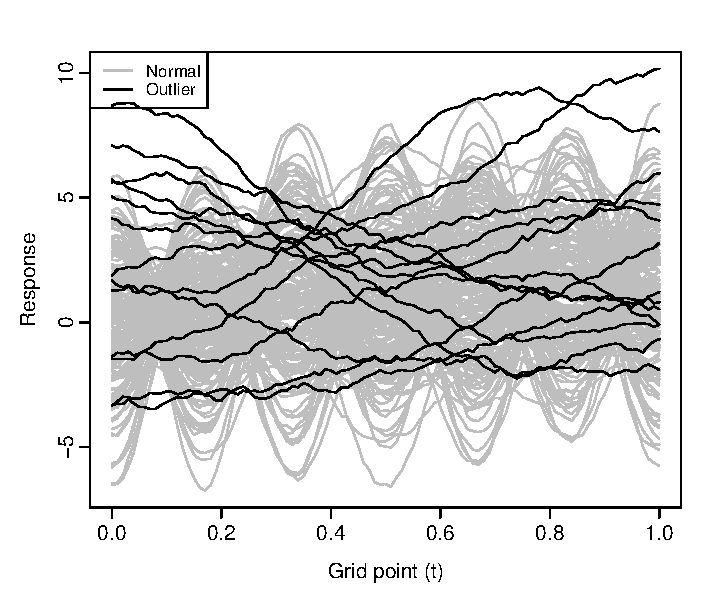
\includegraphics[width=0.46\textwidth]{robflreg-020}
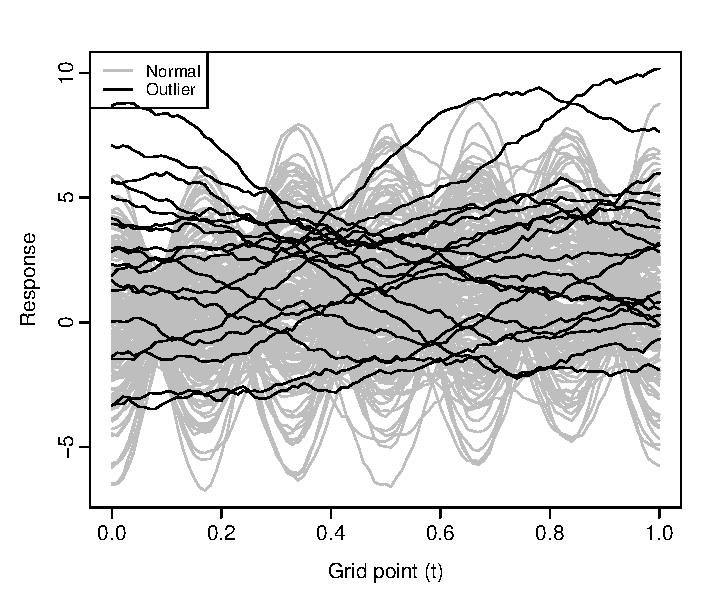
\includegraphics[width=0.46\textwidth]{robflreg-021}
\end{center}
\caption{Plots of the functional response and detected outliers: Classical method (left panel) vs. Robust method (right panel). The detected outlying curves are denoted by black, while the non-outlying curves are denoted by grey.}\label{fig:6}
\end{figure}

The following code can produce the results and Figure~\ref{fig:6}.
\begin{smallexample}
\begin{smallverbatim}
library(robflreg)
# Generate a dataset with five functional predictors and 200
# observations at 101 equally spaced point in the interval [0, 1]
# for each variable for the function-on-function regression model
set.seed(202)
sim.data <- generate.ff.data(n.pred = 5, n.curve = 200, n.gp = 101, out.p = 0.1)
out.indx <- sim.data\$out.indx
# Response variable
Y <- sim.data\$Y
# Predictors
X <- sim.data\$X

gpY = seq(0, 1, length.out = 101) # grid points of Y
gpX <- rep(list(seq(0, 1, length.out = 101)), 5) # grid points of Xs

# Perform classical functional principal component regression using least-squares
model.classical <- rob.ff.reg(Y = Y, X = X, model = "full", emodel = "classical",
                              gpY = gpY, gpX = gpX)

# Perform robust functional principal component regression using MM-estimator
model.MM <- rob.ff.reg(Y = Y, X = X, model = "full", emodel = "robust", fmodel = "MM",
                       gpY = gpY, gpX = gpX)

# Detect outliers using rob.out.detect function
rob.out.detect(object = model.classical, fplot = TRUE)
# outlying functions are: 16 56 69 70 71 80 92 96 117 138 140 173 188
rob.out.detect(object = model.MM, fplot = TRUE)
# outlying functions are: 2 16 56 69 70 71 80 82 92 96 117 134 138 140 
# 173 188 197 199

# Compare with the original outliers
sort(out.indx)
# [1] 2 16 47 56 69 70 71 80 82 92 96 117 134 138 140 162 173 188 197 199
\end{smallverbatim}
\end{smallexample}

\section{Prediction}

We review the prediction problem for a new set of functional predictors based on a fitted functional principal component regression model.

\subsection*{Prediction for the SFRM}

When robustly predicting the unknown values of the scalar response variable for a given new set of functional predictors ($\mathcal{X}^*(s)$), the principal component scores of the new set of functional predictors ($\xi^*$) are obtained as follows:
\begin{equation*}
\xi_{pk}^* = \int_0^1 \mathcal{X}^*_{pk}(s) \widehat{\psi}_{pk}(s) ds,
\end{equation*}
where $\widehat{\psi}_{pk}(s)$ is the $k$-th eigenfunction of the $p$-the functional predictor obtained by the RFPCA. Then, the predictions corresponding to the new set of functional predictors are obtained as follows:
\begin{equation*}
\widehat{Y}^* = \sum_{p=1}^P \sum_{k=1}^{K_p} \widehat{b}_{pk} \xi_{pk}^*,
\end{equation*}
where $\widehat{b}_{pk}$ is the estimated parameter vector obtained from the fitted model \texttt{rob.sf.reg()}.

\subsubsection*{Main function for the robust prediction of a SFRM and its arguments}

The main function for the robust prediction of a SFRM is called \texttt{predict\_sf\_regression()}:
\begin{smallexample}
\begin{smallverbatim}
predict_sf_regression(object, Xnew, Xnew.scl = NULL)
\end{smallverbatim}
\end{smallexample}
In the function \texttt{predict\_sf\_regression()}, the argument \texttt{object} is an output object obtained from \texttt{rob.sf.reg}. The new set of functional predictors is provided in the \texttt{Xnew} argument as a list object whose $p$-th element is a matrix denoting the new observations of $\mathcal{X}_p(s)$. \texttt{Xnew} must have the same length and the same structure as the input \texttt{X} of \texttt{rob.sf.reg}. If scalar predictors are used in the SFRM, then, in the prediction process, the new set of scalar predictors is provided as a matrix in the \texttt{Xnew.scl} argument. The argument
\texttt{Xnew.scl} must have the same length and the same structure as the input \texttt{X.scl} of \texttt{rob.sf.reg}.

To evaluate the prediction performance of classical and robust methods, we simulate a dataset with size $n = 400$ for the SFRM. Then, the simulated data are divided into a training sample with a size of 280 and a test sample with a size of 120. Random outliers contaminate the training sample, and both the classical and robust methods with the tau estimator are applied to the training sample to predict the values of the response variable in the test sample. To compare both methods, we compute the mean squared prediction error (MSPE):
\begin{equation*}
\text{MSPE} = \frac{1}{200} \sum_{i=1}^{200} (Y_i^* - \widehat{Y}_i^*)^2,
\end{equation*}
where $Y_i^*$ and $\widehat{Y}_i^*$ denote the observed and predicted values of the scalar response in the test sample. Our results indicate that the robust method considerably outperforms the classical method. The MSPE computed from the classical method is 20.9388, while the MSPE obtained from the robust method is 1.868. The reproducible code to obtain those results is as follows:
\begin{smallexample}
\begin{smallverbatim}
library(robflreg)
# Generate a dataset with five functional predictors and 400
# observations at 101 equally spaced point in the interval [0, 1]
# for each variable for the scalar-on-function regression model
set.seed(202)
sim.data <- generate.sf.data(n = 400, n.pred = 5, n.gp = 101, out.p = 0.1)
out.indx <- sim.data\$out.indx
# Response variable
Y <- sim.data\$Y
# Predictors
X <- sim.data\$X

# Split the data into training and test samples.
indx.test <- sample(c(1:400)[-out.indx], 120)
indx.train <- c(1:400)[-indx.test]

Y.train <- Y[indx.train,]
Y.test <- Y[indx.test,]
X.train <- X.test <- list()
for(i in 1:5){
  X.train[[i]] <- X[[i]][indx.train,]
  X.test[[i]] <- X[[i]][indx.test,]
}

gp <- rep(list(seq(0, 1, length.out = 101)), 5) # grid points of Xs

# Perform classical functional principal component regression model using training samples
model.classical <- rob.sf.reg(Y.train, X.train, emodel = "classical", gp = gp)
# Perform robust functional principal component regression model 
# using training samples and tau-estimator
model.tau <- rob.sf.reg(Y.train, X.train, emodel = "robust", fmodel = "tau", gp = gp)
# Predict the observations in Y.test using model.classical
pred.classical <- predict_sf_regression(object = model.classical, Xnew = X.test)
# Predict the observations in Y.test using model.tau
pred.tau <- predict_sf_regression(object = model.tau, Xnew = X.test)
# Compute mean squared errors for the test sample
round(mean((Y.test - pred.classical)^2), 4) # 2.49 (classical method)
round(mean((Y.test - pred.tau)^2), 4) # 1.1457 (tau method)
\end{smallverbatim}
\end{smallexample}

\subsection*{Prediction for the FFRM}

In the robust prediction of the FFRM for a given new set of functional predictors, as in the scalar-on-function regression case, the principal component scores of the new set of functional predictors are first obtained:
\begin{equation*}
\xi_{pk}^* = \int_0^1 \mathcal{X}^*_{pk}(s) \widehat{\psi}_{pk}(s) ds,
\end{equation*}
where $\widehat{\psi}_{pk}(s)$ is the $k$-th eigenfunction of the $p$-the functional predictor obtained by the RFPCA. Then, the predictions of functional response ($\widehat{\mathcal{Y}}(t)$) corresponding to the new set of functional predictors are obtained as follows:
\begin{equation*}
\widehat{\mathcal{Y}}^*(t) = \sum_{k=1}^K \left(\sum_{p=1}^P \sum_{j=1}^{K_p} \widehat{b}_{pkj} \xi_{pj}^* \right) \widehat{\phi}_k(t),
\end{equation*}
where $\widehat{\phi}_k(t)$ is the $k$-th eigenfunction of the functional response obtained by RFPCA and $\widehat{b}_{pkj}$ is the estimated parameter matrix obtained from the fitted model \texttt{rob.ff.reg()}.

\subsubsection*{Main function for the robust prediction of a FFRM and its arguments}

The main function for the robust prediction of a FFRM is called \texttt{predict\_ff\_regression()}:
\begin{smallexample}
\begin{smallverbatim}
predict_ff_regression(object, Xnew)
\end{smallverbatim}
\end{smallexample}
Here, the argument \texttt{object} is an output object obtained from \texttt{rob.ff.reg}. The new set of functional predictors is provided in the \texttt{Xnew} argument as a list object whose $p$-th element is a matrix denoting the new observations of $\mathcal{X}_p(s)$. \texttt{Xnew} must have the same length and the same structure as the input \texttt{X} of \texttt{rob.ff.reg}.

We simulate a dataset with size $n = 200$ for the FFRM to investigate and compare the prediction performance of the classical and robust methods. The simulated data are divided into a training sample with a size of 140 and a test sample with a size of 60. Random outliers contaminate the training sample, and both the classical and robust methods with MM estimator are applied to the training sample to predict the values of the response variable in the test sample. To compare both methods, we compute the following MSPE:
\begin{equation*}
\text{MSPE} = \frac{1}{100} \sum_{i=1}^{200} \Vert \mathcal{Y}_i^*(t) - \widehat{\mathcal{Y}}_i^*(t)) \Vert^2_{\mathcal{L}_2},
\end{equation*}
where $\mathcal{Y}_i^*(t)$ and $\widehat{\mathcal{Y}}_i^*(t))$ denote the observed and predicted values of the functional response in the test sample. Our results show that the robust method produces a significantly smaller MSPE value than the classical method. The MSPE computed from the classical method is 3.3213, while the MSPE obtained from the robust method is 0.5925. The reproducible code to obtain those results is as follows:
\begin{smallexample}
\begin{smallverbatim}
library(robflreg)
# Generate a dataset with five functional predictors and 200
# observations at 101 equally spaced point in the interval [0, 1]
# for each variable for the function-on-function regression model
set.seed(202)
sim.data <- generate.ff.data(n.pred = 5, n.curve = 200, n.gp = 101, out.p = 0.1)
out.indx <- sim.data\$out.indx
# Response variable
Y <- sim.data\$Y
# Predictor variables
X <- sim.data\$X
# Split the data into training and test samples.
indx.test <- sample(c(1:200)[-out.indx], 60)
indx.train <- c(1:200)[-indx.test]
Y.train <- Y[indx.train,]
Y.test <- Y[indx.test,]
X.train <- X.test <- list()
for(i in 1:5){
  X.train[[i]] <- X[[i]][indx.train,]
  X.test[[i]] <- X[[i]][indx.test,]
}

gpY = seq(0, 1, length.out = 101) # grid points of Y
gpX <- rep(list(seq(0, 1, length.out = 101)), 5) # grid points of Xs

# Perform classical functional principal component regression model using training samples
model.classical <- rob.ff.reg(Y = Y.train, X = X.train, model = "full",
                              emodel = "classical", gpY = gpY, gpX = gpX)
# Perform robust functional principal component regression 
# using training samples and MM-estimator
model.MM <- rob.ff.reg(Y = Y.train, X = X.train, model = "full", emodel = "robust",
                       fmodel = "MM", gpY = gpY, gpX = gpX)
# Predict the functions in Y.test using model.classical
pred.classical <- predict_ff_regression(object = model.classical, Xnew = X.test)
# Predict the functions in Y.test using model.MM
pred.MM <- predict_ff_regression(object = model.MM, Xnew = X.test)
# Compute mean squared errors for the test sample
round(mean((Y.test - pred.classical)^2), 4) # 1.5705 (classical method)
round(mean((Y.test - pred.MM)^2), 4) # 0.8166 (MM method)
\end{smallverbatim}
\end{smallexample}

\section{Data analysis}

We consider the MaryRiverFlow dataset available in the \pkg{robflreg} package to present the superiority of the robust functional principal component regression models over the classical model when the dataset includes outliers. The MaryRiverFlow dataset consists of hourly river-flow measurements obtained from January 2009 to December 2014 (6 years in total) in the Mary River, Australia. River-flow time series varies throughout the years due to the variation of the seasons and the amount of rainfall received at particular catchments. This problem still needs to be solved in the hydrological domain to be addressed appropriately using theoretical models.

Our first aim with the MaryRiverFlow dataset is to assess how the previous river flow curve time series, $\mathcal{X}_i(s)$, affects the current day's maximum river flow, $Y_i$. Here, the observations of predictor are assumed to be functions of hours, i.e., there are 2188 functional observations $\mathcal{X}_i(t) \big(1\leq t\leq 24$,$~ i=1, \ldots, 2188 \big)$ while the response is a scalar predictor. A graphical display of the response and predictor is presented in Figure~\ref{fig:7}. From this figure, both the scalar response and functional predictor include clear outliers, which motivates us to apply the robust functional principal component regression models to better model this dataset.

\begin{figure}[!htb]
  \begin{center}
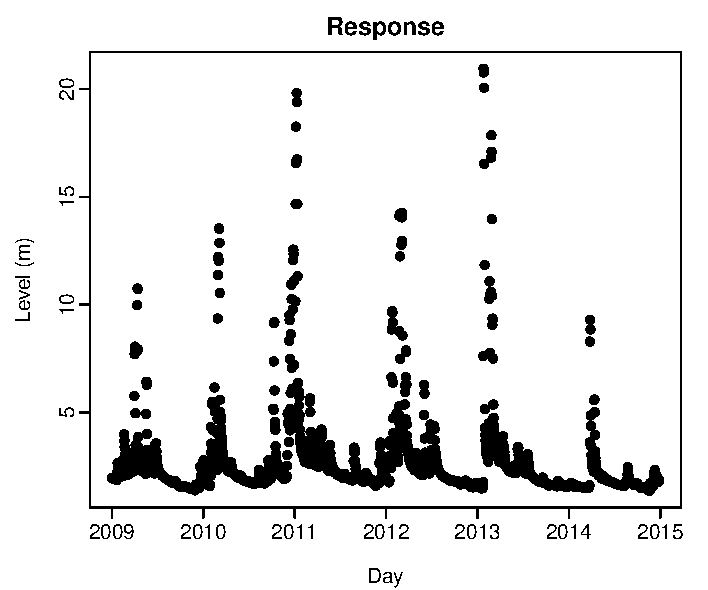
\includegraphics[width=0.49\textwidth]{robflreg-022}
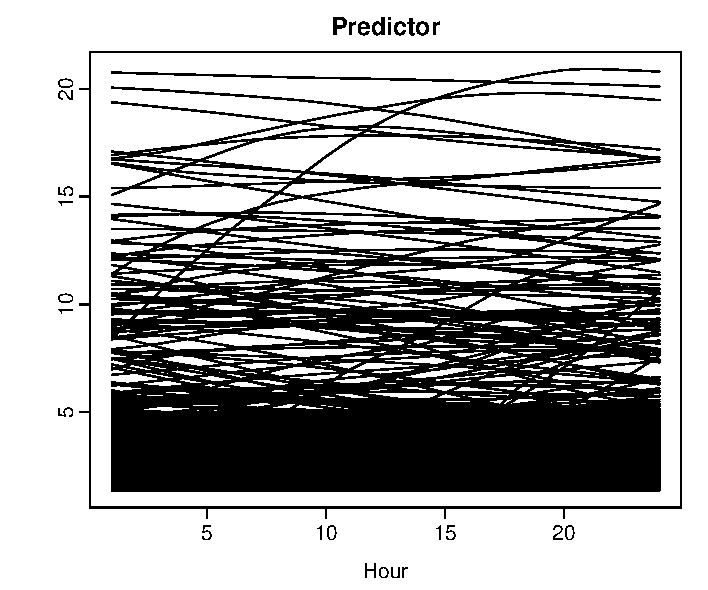
\includegraphics[width=0.49\textwidth]{robflreg-023}
\end{center}
\caption{Plot of the daily maximum river flow measurement (left panel) and the functional time series plot (right panel) of the flow level in the Mary River.}\label{fig:7}
\end{figure}

Figure~\ref{fig:7} can be produced by the following code:
\begin{smallexample}
\begin{smallverbatim}
library(robflreg)
library(fda.usc)
data("MaryRiverFlow")
X <- MaryRiverFlow[1:2188,]
Y <- apply(MaryRiverFlow[2:2189,], 1, max)
Day <- seq(as.Date("2009/01/01"), as.Date("2014/12/28"), by="days")
plot(Day, Y, type = "p", pch = 16, ylab = "Level (m)", main = "Response")
X <- fdata(X, argvals = 1:24)
plot(X, lty = 1, ylab = "", xlab = "Hour", col = "black",
     main = "Predictor", mgp = c(2, 0.5, 0))
\end{smallverbatim}
\end{smallexample}

We assume the SFLRM, $Y_i = \beta_0 + \int \mathcal{X}_i(s) \beta(s) ds$, where $Y_i$ is the maximum river flow measurement for the current day and $\mathcal{X}_i(s)$ is the true river flow measurements recorded in the previous day. An expanding-window approach is considered to compare the predictive performance of the robust methods with the classical one. While doing so, The entire data are divided into two parts: a training sample containing the days from 01/01/2009 to 20/12/2014 and a test sample including days from 21/12/2014 to 30/12/2014. First, the models are constructed using the entire training data to forecast the maximum river flow measurement on 21/12/2014. Then, the maximum river flow measurement is forecasted by increasing the training samples by one day. This procedure is repeated until the training samples cover the entire dataset. The MSPE is computed for each method, and the computed mean MSPEs ($\times 10^{-3}$) along with standard errors ($\times 10^{-3}$ given in bracket) are 7.559 (5.674), 1.635 (1.303), 1.671 (1.376), 1.617 (1.274), and 1.617 (1.274) for the classical, LTS, MM, S, and tau-estimator based SFLRM, respectively. From the results, all the robust methods produce significantly smaller MSPE values than the classical method. These results can be obtained by the following code:
\begin{smallexample}
\begin{smallverbatim}
library(robflreg)
data("MaryRiverFlow")
MaryRiverFlow <- as.matrix(MaryRiverFlow)
X <- list(MaryRiverFlow[1:2188,])
Y <- apply(MaryRiverFlow[2:2189,], 1, max)
gp <- rep(list(1:24), 1)

MSPE <- matrix(, ncol = 5, nrow = 10)
colnames(MSPE) <- c("classical","LTS","MM","S","tau")
starting_value <- 2178

for(i in 1:10){

	# Divide the data into training and test samples
    Y.train <- Y[1:starting_value]
    Y.test <- Y[(starting_value+1)]
    
    X.train <- list(X[[1]][1:starting_value,])
    X.test <- list(matrix(X[[1]][(starting_value+1),], nrow = 1))
    
    # Perform classical and robust functional principal component regression models
    model.classical <- rob.sf.reg(Y.train, X.train, emodel = "classical", gp = gp)
    model.LTS <- rob.sf.reg(Y.train, X.train, emodel = "robust", fmodel = "LTS", gp = gp)
    model.MM <- rob.sf.reg(Y.train, X.train, emodel = "robust", fmodel = "MM", gp = gp)
    model.S <- rob.sf.reg(Y.train, X.train, emodel = "robust", fmodel = "S", gp = gp)
    model.tau <- rob.sf.reg(Y.train, X.train, emodel = "robust", fmodel = "tau", gp = gp)
    
    # Predict the maximum river flow measurement of the current day
    pred.classical <- predict_sf_regression(object = model.classical, Xnew = X.test)
    pred.LST <- predict_sf_regression(object = model.LTS, Xnew = X.test)
    pred.MM <- predict_sf_regression(object = model.MM, Xnew = X.test)
    pred.S <- predict_sf_regression(object = model.tau, Xnew = X.test)
    pred.tau <- predict_sf_regression(object = model.tau, Xnew = X.test)
    
    # Record the MSPE values
    MSPE[i,1] <- (Y.test - pred.classical)^2
    MSPE[i,2] <- (Y.test - pred.LST)^2
    MSPE[i,3] <- (Y.test - pred.MM)^2
    MSPE[i,4] <- (Y.test - pred.S)^2
    MSPE[i,5] <- (Y.test - pred.tau)^2
    starting_value <- starting_value + 1
}

apply(MSPE, 2, mean); apply(MSPE, 2, sd)
\end{smallverbatim}
\end{smallexample}

Our second aim with the MaryRiverFlow dataset is to assess how the previous river flow curve time series, $\mathcal{X}_i(s)$ affects the current day's river flow curve time series, $\mathcal{Y}_i(t)$. In this case, the elements of both the response and predictor are assumed to be functions of hours. Here, we assume the FFLRM, $\mathcal{Y}_i(t) = \beta_0(t) + \int \mathcal{X}_i(s) \beta(s,t) ds dt$. The similar expanding-window approach used in the SFLRM example is considered, i.e., the entire dataset is divided into two parts: a training sample containing the days from 01/01/2009 to 20/12/2014 and a test sample including days from 21/12/2014 to 30/12/2014. The functional principal component regression models are constructed using the entire training data to forecast the river flow curve time series on 21/12/2014. Then, the river flow curve time series is forecasted by increasing the training samples by one day. This procedure is repeated until the training samples cover the entire dataset. The MSPE is computed for each method, and the computed mean MSPEs ($\times 10^{-3}$) along with standard errors ($\times 10^{-3}$ given in bracket) are 5.721 (3.884), 1.565 (0.965), 1.377 (0.847), 1.546 (0.949), 1.511 (0.920), and 1.377 (0.849) for the classical, MCD, MLTS, MM, S, and tau-estimator based FFLRMs, respectively. From the results, the robust methods produce improved MSPEs over the classical FFLRM, i.e., the robust method models the MaryRiverFlow data better than the classical functional principal component regression model. These results can be obtained by the following code:
\begin{smallexample}
\begin{smallverbatim}
library(robflreg)
data("MaryRiverFlow")
MaryRiverFlow <- as.matrix(MaryRiverFlow)

# The following function is used to obtain the functional response and predictor
var_fun = function(data,order){
  n = dim(data)[1]
  y = data[((order+1):n),]
  x=list()
  a=1
  b=order
  for(i in 1:order){
    x[[i]] = data[(a:(n-b)),]
    a = a+1
    b = b-1
  }
  return(list(x=x,y=y))
}

# Grid points for the functional response and predictor
gpY <- 1:24 # grid points of Y
gpX <- rep(list(1:24), 1) # grid points of Xs

MSPE <- matrix(, ncol = 6, nrow = 10)
colnames(MSPE) <- c("classical","MCD","MLTS","MM","S","tau")
starting_value <- 2179
# In two cases (when i = 3 and i = 6) the covariance is not decomposed.
# Thus, try() is used to ignore these two cases.
for(i in 1:10){
  try({
  data.i <- MaryRiverFlow[1:starting_value,]
  # Obtain the functional response and predictor
  XY = var_fun(data=data.i, order=1)
  X = XY$x
  Y = XY$y

  # Perform classical and robust functional principal component regression models
  model.classical <- rob.ff.reg(Y = Y, X = X, model = "full", emodel = "classical",
                         gpY = gpY, gpX = gpX)
  model.MCD <- rob.ff.reg(Y = Y, X = X, model = "full", emodel = "robust",
                         fmodel = "MCD", gpY = gpY, gpX = gpX)
  model.MLTS <- rob.ff.reg(Y = Y, X = X, model = "full", emodel = "robust",
                         fmodel = "MLTS", gpY = gpY, gpX = gpX)
  model.MM <- rob.ff.reg(Y = Y, X = X, model = "full", emodel = "robust",
                         fmodel = "MM", gpY = gpY, gpX = gpX)
  model.S <- rob.ff.reg(Y = Y, X = X, model = "full", emodel = "robust",
                         fmodel = "S", gpY = gpY, gpX = gpX)
  model.tau <- rob.ff.reg(Y = Y, X = X, model = "full", emodel = "robust",
                         fmodel = "tau", gpY = gpY, gpX = gpX)
  Xnew = list(t(as.matrix(Y[dim(Y)[1],])))
  
  # Predict the maximum river flow measurement of the current day
  predict.classical <- predict_ff_regression(object = model.classical, Xnew = Xnew)
  predict.MCD <- predict_ff_regression(object = model.MCD, Xnew = Xnew)
  predict.MLTS <- predict_ff_regression(object = model.MLTS, Xnew = Xnew)
  predict.MM <- predict_ff_regression(object = model.MM, Xnew = Xnew)
  predict.S <- predict_ff_regression(object = model.S, Xnew = Xnew)
  predict.tau <- predict_ff_regression(object = model.tau, Xnew = Xnew)

  # Record the MSPE values
  MSPE[i,1] <- mean((predict.classical - MaryRiverFlow[starting_value+1,])^2)
  MSPE[i,2] <- mean((predict.MCD - MaryRiverFlow[starting_value+1,])^2)
  MSPE[i,3] <- mean((predict.MLTS - MaryRiverFlow[starting_value+1,])^2)
  MSPE[i,4] <- mean((predict.MM - MaryRiverFlow[starting_value+1,])^2)
  MSPE[i,5] <- mean((predict.S - MaryRiverFlow[starting_value+1,])^2)
  MSPE[i,6] <- mean((predict.tau - MaryRiverFlow[starting_value+1,])^2)
  starting_value <- starting_value +1
  },silent=T)
}

apply(MSPE, 2, mean, na.rm=TRUE); apply(MSPE, 2, sd, na.rm=TRUE)
\end{smallverbatim}
\end{smallexample}

\section{Conclusion}

The \textsf{R} package \pkg{robflreg} provides an implementation of functional principal component regression model based on several robust procedures to fit and predict SFLRM and FFLRM. These methods are centered on the RFPCA of \cite{Bali2011}, a popular robust dimension reduction technique in functional data, and several robust regression parameter estimators. In addition, the package \pkg{robflreg} allows us to fit and predict SFLRM and FFLRM via the classical FPCA and least-squares estimator. Several simulation examples and empirical data analysis show that the robust procedures provide better inference for functional linear regression models when outliers are present in the response and predictor variables. The \pkg{robflreg} package code can be found at: \url{https://github.com/cran/robflreg}.

The aspects that the current version of the \texttt{R} package \pkg{robflreg} that may be improved upon in the future are listed below.
\begin{enumerate}
\item[1)] In the current version, the scalar predictors are allowed in the SFLRM only. In the next versions of the package, it is planned to improve the functions \texttt{rob.ff.reg} and \texttt{predict\_ff\_regression} to include scalar predictors (whose effects are constant and/or vary along the continuum of the functional predictor).
\item[2)] The current package version does not allow for modeling the function-on-scalar regression model, where the response consists of random functions, and the predictors include scalar observations. The robust procedures used in the FFLRM are planned to extend the function-on-scalar regression model in the subsequent versions of the package.
\item[3)] In the current version, the observations of the functional variables are assumed to be densely observed. In the next versions of the package, the robust methods are planned to extend the models where the elements of functional variables can also be observed over irregular and curve-specific grids.
\end{enumerate}

\section*{Acknowledgement}

We thank three reviewers for their careful reading of our manuscript and valuable suggestions and comments, which have helped us produce an improved version of our manuscript and the \texttt{R} package. The first author was supported by The Scientific and Technological Research Council of Turkey (TUBITAK) (grant no: 120F270). The second author was partially supported by an Australian Research Council Discovery Project (grant no: DP230102250). This study is dedicated to the people who lost their lives in the earthquake that occurred in Turkey on February 6, 2023.

\bibliography{betaztas-shang}

\address{Ufuk Beyaztas\\
  Marmara University\\
  Department of Statistics, Goztepe Campus, 34722, Kadikoy, Istanbul\\
  Turkey\\
  (ORCID 0000-0002-5208-4950)\\
  \email{ufuk.beyaztas@marmara.edu.tr}}

\address{Han Lin Shang\\
  Macquarie University\\
  Department of Actuarial Studies and Business Analytics, Level 7, 4 Eastern Road, Sydney, NSW 2109\\
  Australia\\
  (ORCID 0000-0003-1769-6430)\\
  \email{hanlin.shang@mq.edu.au}}
